\documentclass[12pt]{article} %try documentclass book

%\usepackage[left=0.5in,right=0.5in, top=0.2in, bottom=0.8in]{geometry}
%\geometry{papersize={6in,9in}}

\usepackage[left=0.625in,right=0.625in, top=0.325in, bottom=0.925in]{geometry}
\geometry{papersize={6.25in,9.25in}}
\linespread{1.3}
\usepackage[most]{tcolorbox}
\usepackage{pgfornament}
\usepackage{lipsum}
\usepackage{transparent}
\usepackage{tikz}
\usepackage{csquotes}
\usepackage{setspace}
\usepackage{calc}

% This is for making text and a blank line until the end of the line. The input is the text, and this adds a blank line after it.
\newlength{\remaining}
\newcommand{\fillinline}[1]{%
\setlength{\remaining}{\textwidth-\widthof{\textsc{#1}}-1.5cm}
\textsc{#1} $\rule{\remaining}{0.15mm}$}

% mypage command creates a new page with the spiffy background
\newcommand{\mypage}{\newpage 
\tikz[remember picture,overlay] 
\node[opacity=0.25,inner sep=0pt] at (-0.6,-0.6)
{
\includegraphics[height=\paperheight]{./Images/Hopf_colour.png}};}

% myquote adds a quote for the quotes page. First input is the quote, second input is the person who said it
\newcommand{\myquote}[2]{
\begin{flushleft}
  \enquote{#1}
\end{flushleft}
\begin{flushright}
  -- #2
\end{flushright}
\begin{center}
  \pgfornament[width=3cm,height=0.3cm]{87}
\end{center}
}

% Boxes and such defined below:

\newtcolorbox{mybox}[1][]{
enhanced,
arc=0pt,
outer arc=0pt,
colback=black!1!white,
colframe=black!50!white,
boxrule=0.8pt,
attach boxed title to top center={yshift=-2mm},
top=20pt,
bottom=10pt,
arc=5pt,
auto outer arc,
#1
}

\newtcolorbox{titlebox}[1][]{
enhanced,
arc=0pt,
outer arc=0pt,
colback=black!1!white,
colframe=black!50!white,
boxrule=0.8pt,
attach boxed title to top center={yshift=-2mm},
top=10pt,
bottom=10pt,
arc=5pt,
auto outer arc,
%nobeforeafter,
%overlay={\node[draw,fill=white,fill opacity=1,inner sep=5mm,rounded corners] at ([xshift=1.5cm,yshift=-0.6cm]frame.north west) {Date:$\rule{0.75cm}{0.15mm}$};},
#1
}

\newtcolorbox{ratebox}[1][]{
enhanced,
arc=0pt,
outer arc=0pt,
colback=black!1!white,
colframe=black!50!white,
boxrule=0.8pt,
attach boxed title to top center={yshift=-5mm},
top=20pt,
bottom=10pt,
arc=5pt,
auto outer arc,
#1
}

\newtcolorbox{listbox}[1][]{
enhanced,
arc=0pt,
outer arc=0pt,
colback=black!1!white,
colframe=black!50!white,
boxrule=0.8pt,
attach boxed title to top center={yshift=-2mm},
top=10pt,
bottom=20pt,
arc=5pt,
auto outer arc,
#1
}

% Teaching toolbox commands

% First input: name
% second input: what is it?
% Third input: variants
% Fourth input: Uses
\newcommand{\addtoolboxitem}[4]{
\mypage
\addcontentsline{toc}{subsection}{#1}
\subsection*{#1}
\vspace{0.25in}
\begin{center}
  \begin{tabular}{rp{3in}}
    \textbf{What it is:}& #2 \\
    \textbf{Possible Variants:}&#3\\
    \textbf{Uses:}& #4\\
    \textbf{Tips\&Tricks:}&
    %\begin{minipage}{\textwidth}
      \setstretch{1.3}
      \vspace{0.3cm}
      $\rule{3in}{0.15mm}$\newline
      $\rule{3in}{0.15mm}$\newline
      $\rule{3in}{0.15mm}$
      \setstretch{1}
    %\end{minipage}
    \\
  \end{tabular}
\end{center}
\vspace*{\fill}
\begin{center}
  \begin{mybox}[width=\textwidth,title={Experiences}]
    \vspace{2in}
  \end{mybox}
\end{center}
}

%blank teaching toolbox item
\newcommand{\addblanktoolboxitem}{
\mypage
\subsection*{$\rule{6cm}{0.15mm}$}
\vspace{0.25in}
\begin{center}
  \begin{tabular}{rp{3in}}
    \textbf{What it is:}& 
        \setstretch{1.3}
        \vspace{0.3cm}
        $\rule{3in}{0.15mm}$\newline
        $\rule{3in}{0.15mm}$\newline
        $\rule{3in}{0.15mm}$
        \setstretch{1} \\
    \textbf{Possible Variants:}&
        \setstretch{1.3}
        \vspace{0.3cm}
        $\rule{3in}{0.15mm}$\newline
        $\rule{3in}{0.15mm}$
        \setstretch{1} \\
    \textbf{Uses:}&
        \setstretch{1.3}
        \vspace{0.3cm}
        $\rule{3in}{0.15mm}$\newline
        $\rule{3in}{0.15mm}$\newline
        $\rule{3in}{0.15mm}$
        \setstretch{1} \\
    \textbf{Tips\&Tricks:}&
    %\begin{minipage}{\textwidth}
      \setstretch{1.3}
      \vspace{0.3cm}
      $\rule{3in}{0.15mm}$\newline
      $\rule{3in}{0.15mm}$\newline
      $\rule{3in}{0.15mm}$
      \setstretch{1}
    %\end{minipage}
    \\
  \end{tabular}
\end{center}
\vspace*{\fill}
\begin{center}
  \begin{mybox}[width=\textwidth,title={Experiences}]
    \vspace{2in}
  \end{mybox}
\end{center}
}

\def \bs{\textbackslash}
\newcommand{\mute}[1]{}

\newcommand{\addlesson}{\mypage
\begin{titlebox}[width=\textwidth]
  \begin{tabular}{rl}
    \textbf{Title:}&$\rule{0.7\textwidth}{0.15mm}$\\
    \textbf{References:}&$\rule{0.7\textwidth}{0.15mm}$\\
    \textbf{Last Class:}&$\rule{0.7\textwidth}{0.15mm}$\\
    \textbf{Next Class:}&$\rule{0.7\textwidth}{0.15mm}$\\
    %\textbf{Last Class:}&$\rule{0.28\textwidth}{0.15mm}$ \textbf{Next Class:} $\rule{0.27\textwidth}{0.15mm}$\\
    %\textbf{Announcements:}&$\rule{0.7\textwidth}{0.15mm}$
  \end{tabular}
\end{titlebox}
\begin{mybox}[width=\textwidth,title=One Sentence Summary]
  \vspace{1cm}
\end{mybox}

\begin{mybox}[width=\textwidth,title=Objectives]%,box align=top]%,watermark text=Goals,watermark opacity=0.7]
  \begin{tabular}{rl}
    \fbox{1}&$\rule{0.87\textwidth}{0.15mm}$\\
            &$\rule{0.87\textwidth}{0.15mm}$\\
    \fbox{2}&$\rule{0.87\textwidth}{0.15mm}$\\
            &$\rule{0.87\textwidth}{0.15mm}$\\
    \fbox{3}&$\rule{0.87\textwidth}{0.15mm}$\\
            &$\rule{0.87\textwidth}{0.15mm}$\\
    \fbox{4}&$\rule{0.87\textwidth}{0.15mm}$\\
            &$\rule{0.87\textwidth}{0.15mm}$\\
    \fbox{5}&$\rule{0.87\textwidth}{0.15mm}$\\
            &$\rule{0.87\textwidth}{0.15mm}$\\
  \end{tabular}
\end{mybox}

\begin{mybox}[title=Teacher Development,width=\textwidth]% box align=top]
  {\small \textbf{I will focus on\bs expect to struggle with\bs am going to try}\\}
  \vspace{1cm}
\end{mybox}

\mypage
\begin{mybox}[width=\textwidth,title={Announcements \& Reminders:}]
\end{mybox}

\begin{mybox}[width=\textwidth,title=Activities]
  \begin{tabular}{p{0.04\textwidth}p{0.8\textwidth}p{0.04\textwidth}}
    \begin{minipage}{0.04\textwidth}
      \rotatebox[origin=c]{90}{\hbox{\transparent{0.4} Objectives 
      related to activity}}
    \end{minipage}
    &
    \begin{minipage}{0.9\textwidth}
    $\rule{0.9\textwidth}{0.15mm}$\\
    $\rule{0.9\textwidth}{0.15mm}$\\
    $\rule{0.9\textwidth}{0.15mm}$\\
    $\rule{0.9\textwidth}{0.15mm}$\\
    $\rule{0.9\textwidth}{0.15mm}$\\
    $\rule{0.9\textwidth}{0.15mm}$\\
    $\rule{0.9\textwidth}{0.15mm}$\\
    $\rule{0.9\textwidth}{0.15mm}$\\
    $\rule{0.9\textwidth}{0.15mm}$\\
    $\rule{0.9\textwidth}{0.15mm}$\\
    $\rule{0.9\textwidth}{0.15mm}$\\
    $\rule{0.9\textwidth}{0.15mm}$\\
    $\rule{0.9\textwidth}{0.15mm}$\\
    $\rule{0.9\textwidth}{0.15mm}$\\
    $\rule{0.9\textwidth}{0.15mm}$\\
    $\rule{0.9\textwidth}{0.15mm}$\\
    $\rule{0.9\textwidth}{0.15mm}$\\
    $\rule{0.9\textwidth}{0.15mm}$\\
    $\rule{0.9\textwidth}{0.15mm}$\\
    $\rule{0.9\textwidth}{0.15mm}$\\
    $\rule{0.9\textwidth}{0.15mm}$\\
    $\rule{0.9\textwidth}{0.15mm}$\\
    $\rule{0.9\textwidth}{0.15mm}$\\
    $\rule{0.9\textwidth}{0.15mm}$\\
  \end{minipage}
  &
  \begin{minipage}{0.04\textwidth}
      \rotatebox[origin=c]{90}{\hbox{\transparent{0.4} Time estimates}}
    \end{minipage}
  \end{tabular}
\end{mybox}
\mypage
\begin{mybox}[width=\textwidth,title=Activities]
  \begin{tabular}{p{0.04\textwidth}p{0.8\textwidth}p{0.04\textwidth}}
    \begin{minipage}{0.04\textwidth}
      \rotatebox[origin=c]{90}{\hbox{\transparent{0.4} Objectives 
      related to activity}}
    \end{minipage}
    &
    \begin{minipage}{0.9\textwidth}
    $\rule{0.9\textwidth}{0.15mm}$\\
    $\rule{0.9\textwidth}{0.15mm}$\\
    $\rule{0.9\textwidth}{0.15mm}$\\
    $\rule{0.9\textwidth}{0.15mm}$\\
    $\rule{0.9\textwidth}{0.15mm}$\\
    $\rule{0.9\textwidth}{0.15mm}$\\
    $\rule{0.9\textwidth}{0.15mm}$\\
    $\rule{0.9\textwidth}{0.15mm}$\\
    $\rule{0.9\textwidth}{0.15mm}$\\
    $\rule{0.9\textwidth}{0.15mm}$\\
    $\rule{0.9\textwidth}{0.15mm}$\\
    $\rule{0.9\textwidth}{0.15mm}$\\
    $\rule{0.9\textwidth}{0.15mm}$\\
    $\rule{0.9\textwidth}{0.15mm}$\\
    $\rule{0.9\textwidth}{0.15mm}$\\
    $\rule{0.9\textwidth}{0.15mm}$\\
    $\rule{0.9\textwidth}{0.15mm}$\\
    $\rule{0.9\textwidth}{0.15mm}$\\
    $\rule{0.9\textwidth}{0.15mm}$\\
    $\rule{0.9\textwidth}{0.15mm}$\\
    $\rule{0.9\textwidth}{0.15mm}$\\
    $\rule{0.9\textwidth}{0.15mm}$\\
    $\rule{0.9\textwidth}{0.15mm}$\\
    $\rule{0.9\textwidth}{0.15mm}$\\
    $\rule{0.9\textwidth}{0.15mm}$\\
    $\rule{0.9\textwidth}{0.15mm}$\\
    $\rule{0.9\textwidth}{0.15mm}$\\
  \end{minipage}
  &
  \begin{minipage}{0.04\textwidth}
      \rotatebox[origin=c]{90}{\hbox{\transparent{0.4} Time estimates}}
    \end{minipage}
  \end{tabular}
\end{mybox}

%\begin{mybox}[width=\textwidth,title=Lecture Summary]
%  \textbf{activity}\hspace{4cm} \textbf{objective} \hspace{2cm}
%  \textbf{time est.}\\
%  $\rule{\textwidth}{0.15mm}$\\
%  $\rule{\textwidth}{0.15mm}$\\
%  $\rule{\textwidth}{0.15mm}$\\
%  $\rule{\textwidth}{0.15mm}$\\
%  $\rule{\textwidth}{0.15mm}$\\
%  $\rule{\textwidth}{0.15mm}$\\
%  $\rule{\textwidth}{0.15mm}$\\
%\end{mybox}
\mypage
\begin{mybox}[width=\textwidth,title={Reflection: Highlights}]
\begin{center}
    $\rule{0.9\textwidth}{0.15mm}$\\
    $\rule{0.9\textwidth}{0.15mm}$\\
    $\rule{0.9\textwidth}{0.15mm}$\\
    $\rule{0.9\textwidth}{0.15mm}$\\
    $\rule{0.9\textwidth}{0.15mm}$\\
    $\rule{0.9\textwidth}{0.15mm}$\\
    $\rule{0.9\textwidth}{0.15mm}$\\
    $\rule{0.9\textwidth}{0.15mm}$
    \end{center}
\end{mybox}

\begin{mybox}[width=\textwidth,title={Reflection: A lesson for next time}]
\begin{center}
    $\rule{0.9\textwidth}{0.15mm}$\\
    $\rule{0.9\textwidth}{0.15mm}$\\
    $\rule{0.9\textwidth}{0.15mm}$\\
    $\rule{0.9\textwidth}{0.15mm}$\\
    $\rule{0.9\textwidth}{0.15mm}$
    \end{center}
\end{mybox}

\begin{mybox}[width=\textwidth,title={Reflection: Targeted Question (see ``Other Resources'')}]
\begin{center}
    $\rule{0.9\textwidth}{0.15mm}$\\
    $\rule{0.9\textwidth}{0.15mm}$\\
    $\rule{0.9\textwidth}{0.15mm}$\\
    $\rule{0.9\textwidth}{0.15mm}$\\
    $\rule{0.9\textwidth}{0.15mm}$
    \end{center}
\end{mybox}

\begin{ratebox}[width=\textwidth,title={Did it live up to my expectations?}]
  \begin{center}
    \begin{tabular}{cccccccccc}
      1&2&3&4&5&6&7&8&9&10
    \end{tabular}
  \textbf{Why?}$\rule{0.9\textwidth}{0.15mm}$
  \end{center}
\end{ratebox}


}

\newcommand{\Repeat}[2]{
    \foreach \n in {1,...,#1}{#2}
}

\begin{document}
%\pagenumbering{gobble}
\tikz[remember picture,overlay] 
\node[opacity=0.25,inner sep=0pt] at (2.5in,-4.1in)
{
\includegraphics[height=0.9\paperheight]{./Images/Hopf_colour.png}};

\vspace{4cm}
\thispagestyle{empty}
\begin{center}
{\Huge \textbf{Teaching Handbook}}\\
\end{center}

\vspace{1cm} \ \\

\begin{center}
  {\Large \textbf{Your one-stop shop for teaching strategies, 
  classroom preparation, and self-assessment}}
\end{center}


\vspace{5cm}\ \\
\begin{center}
\textbf{Designed, composed, and written by the 2019-2020 Calculus Community of Practice at the University of Toronto.}
\end{center}
\newpage

\thispagestyle{empty}

\tikz[remember picture,overlay] 
\node[opacity=0.25,inner sep=0pt] at (2.5in,-4.1in)
{
\includegraphics[height=0.9\paperheight]{./Images/Hopf_colour.png}};
\newpage

\setcounter{page}{1}
\tikz[remember picture,overlay] 
\node[opacity=0.25,inner sep=0pt] at (-0.6,-0.6)
{
\includegraphics[height=\paperheight]{./Images/Hopf_colour.png}};

\vspace{4cm}
\begin{center}
{\Large \textbf{Teaching Handbook}}\\
\vspace{3cm}\ \\
\textbf{Designed, composed, and written by the 2019-2020 Calculus Community of Practice at the University of Toronto.}
  \begin{center}
    
\includegraphics[width=5cm]{./Images/logo.png}
  \end{center}
\end{center}


\mypage
\mypage
\vspace{-1.5cm}
\tableofcontents
\mypage
\mypage
\addcontentsline{toc}{section}{Calendar}

\vspace{6cm}
\begin{center}
{\Large \textbf{Calendar}}
\end{center}
\mypage
\begin{mybox}[width=\textwidth]

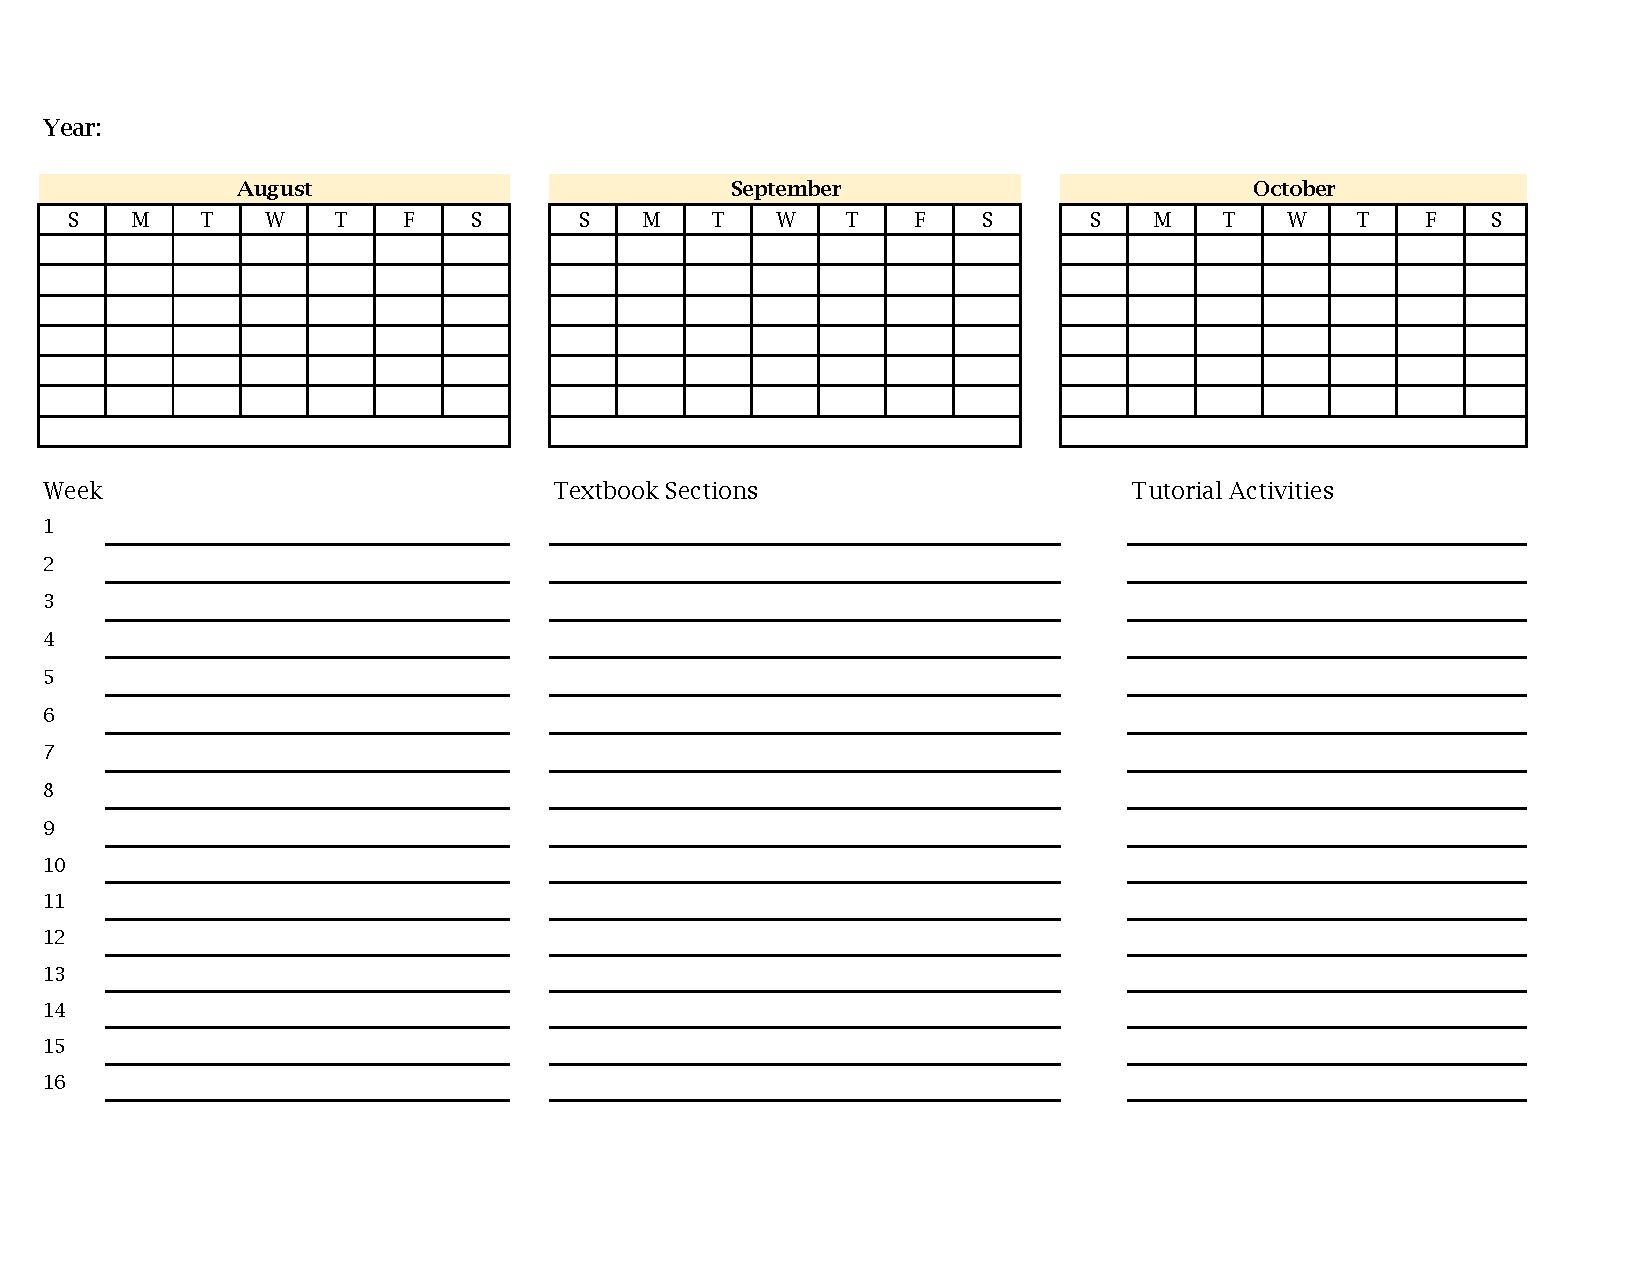
\includegraphics[width=4.5in,height=7in]{Calendar1.pdf}

\end{mybox}
\mypage

\begin{mybox}[width=\textwidth]

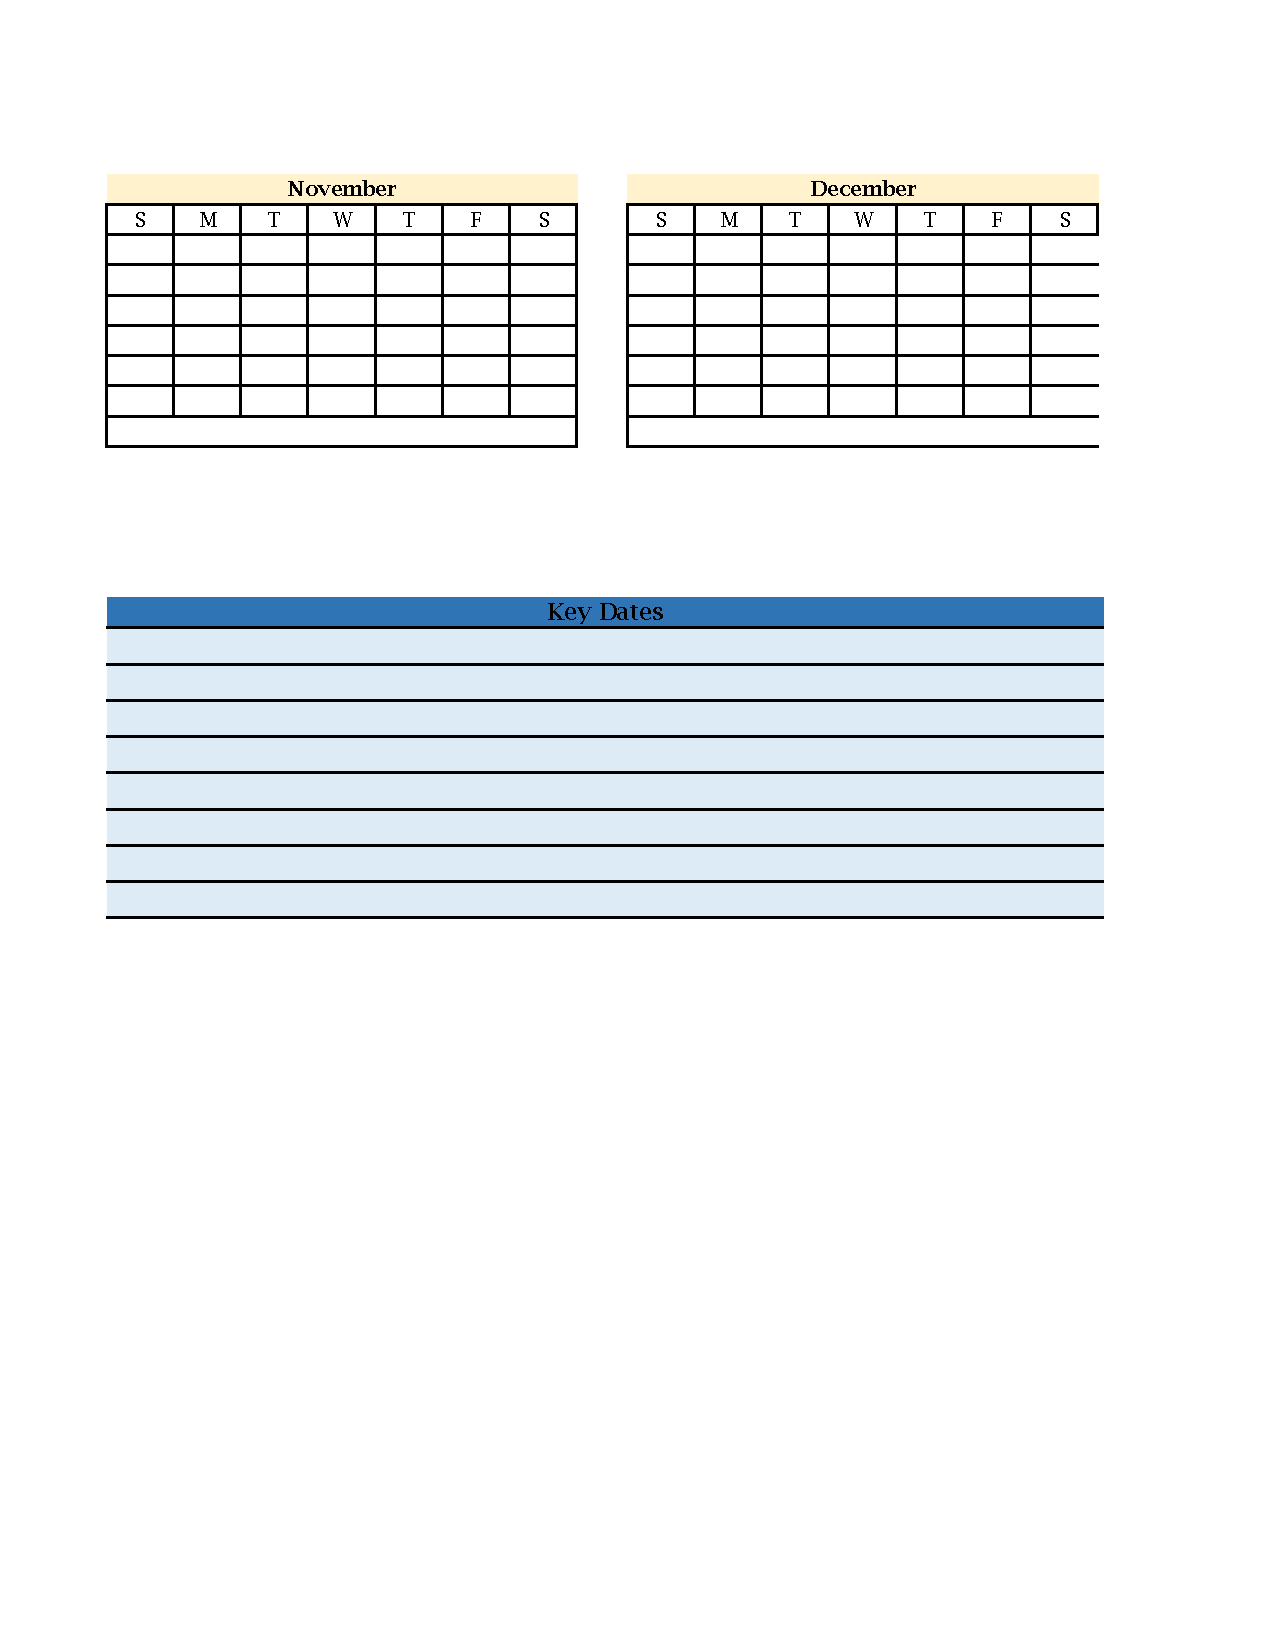
\includegraphics[width=4.5in,height=7in]{Calendar2.pdf}

\end{mybox}

\mypage

\begin{mybox}[width=\textwidth]

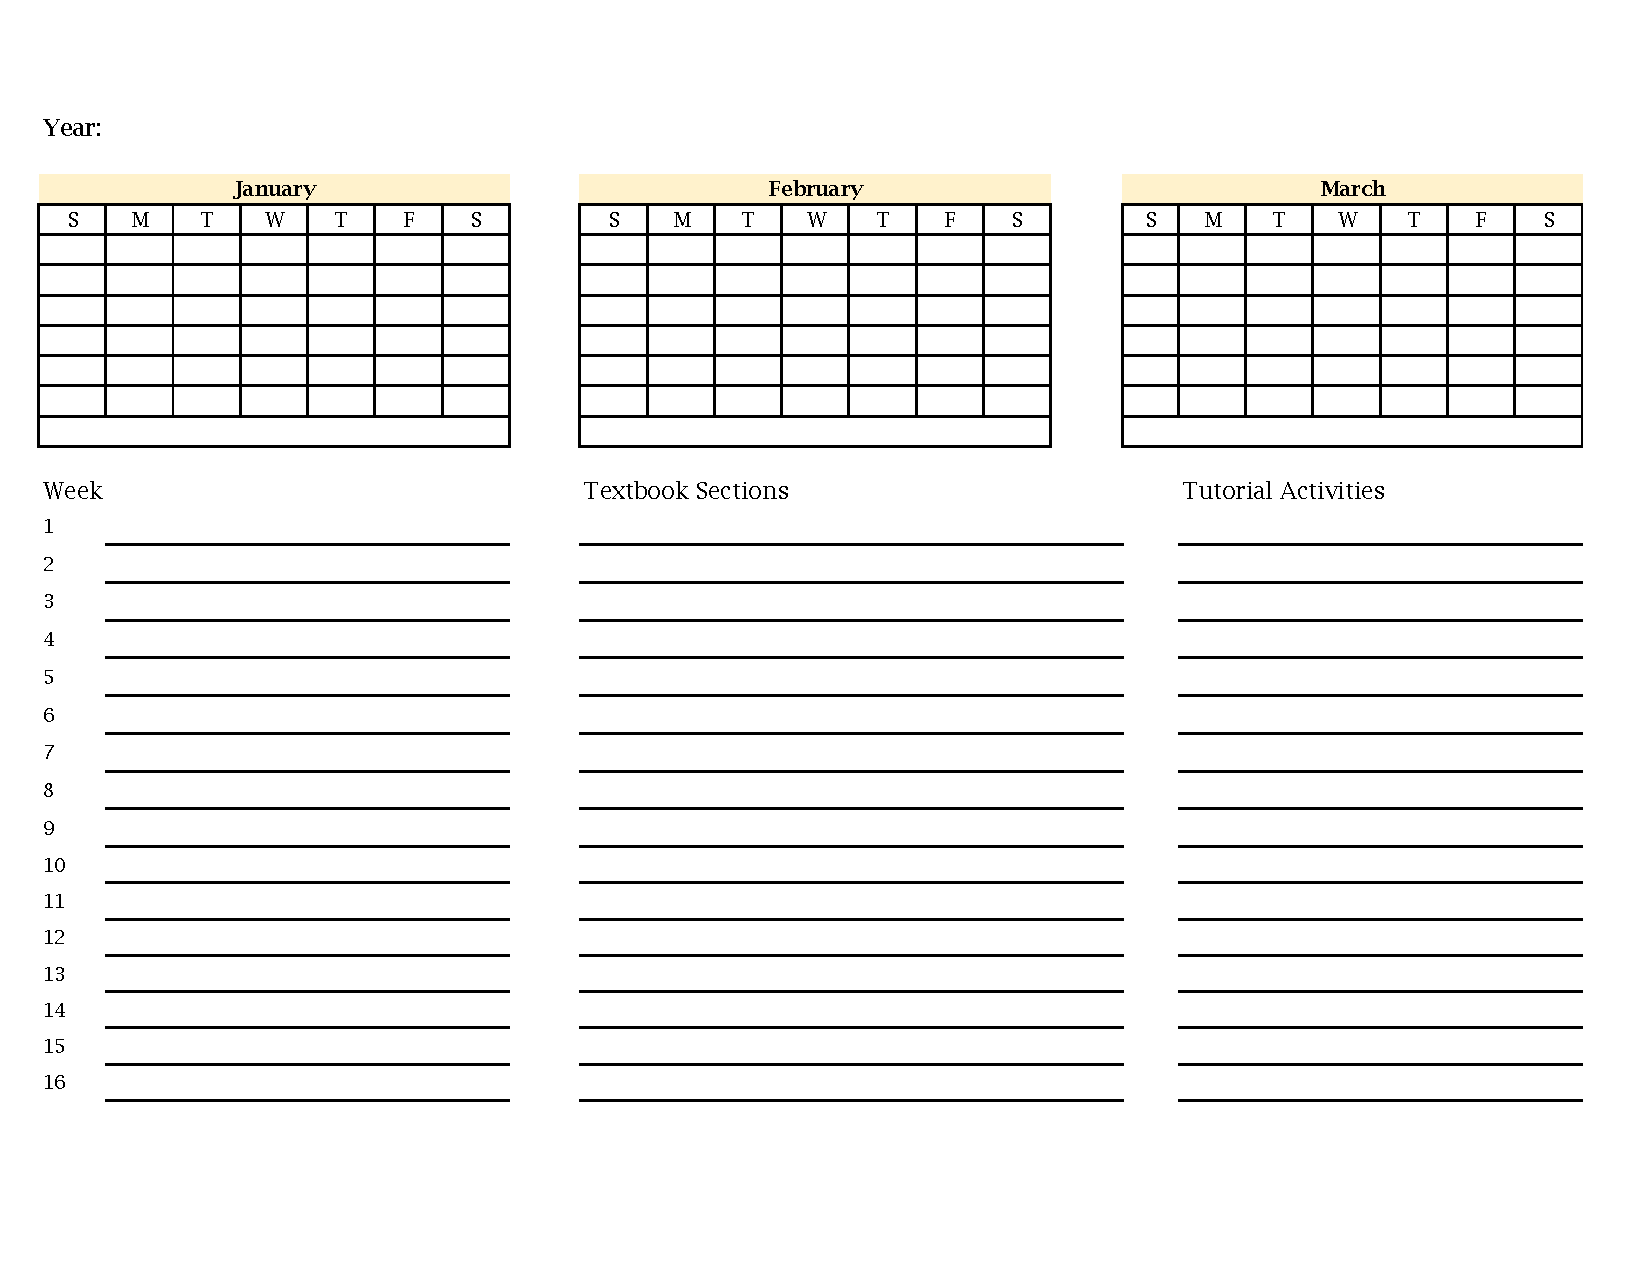
\includegraphics[width=4.5in,height=7in]{Calendar3.pdf}

\end{mybox}

\mypage

\begin{mybox}[width=\textwidth]

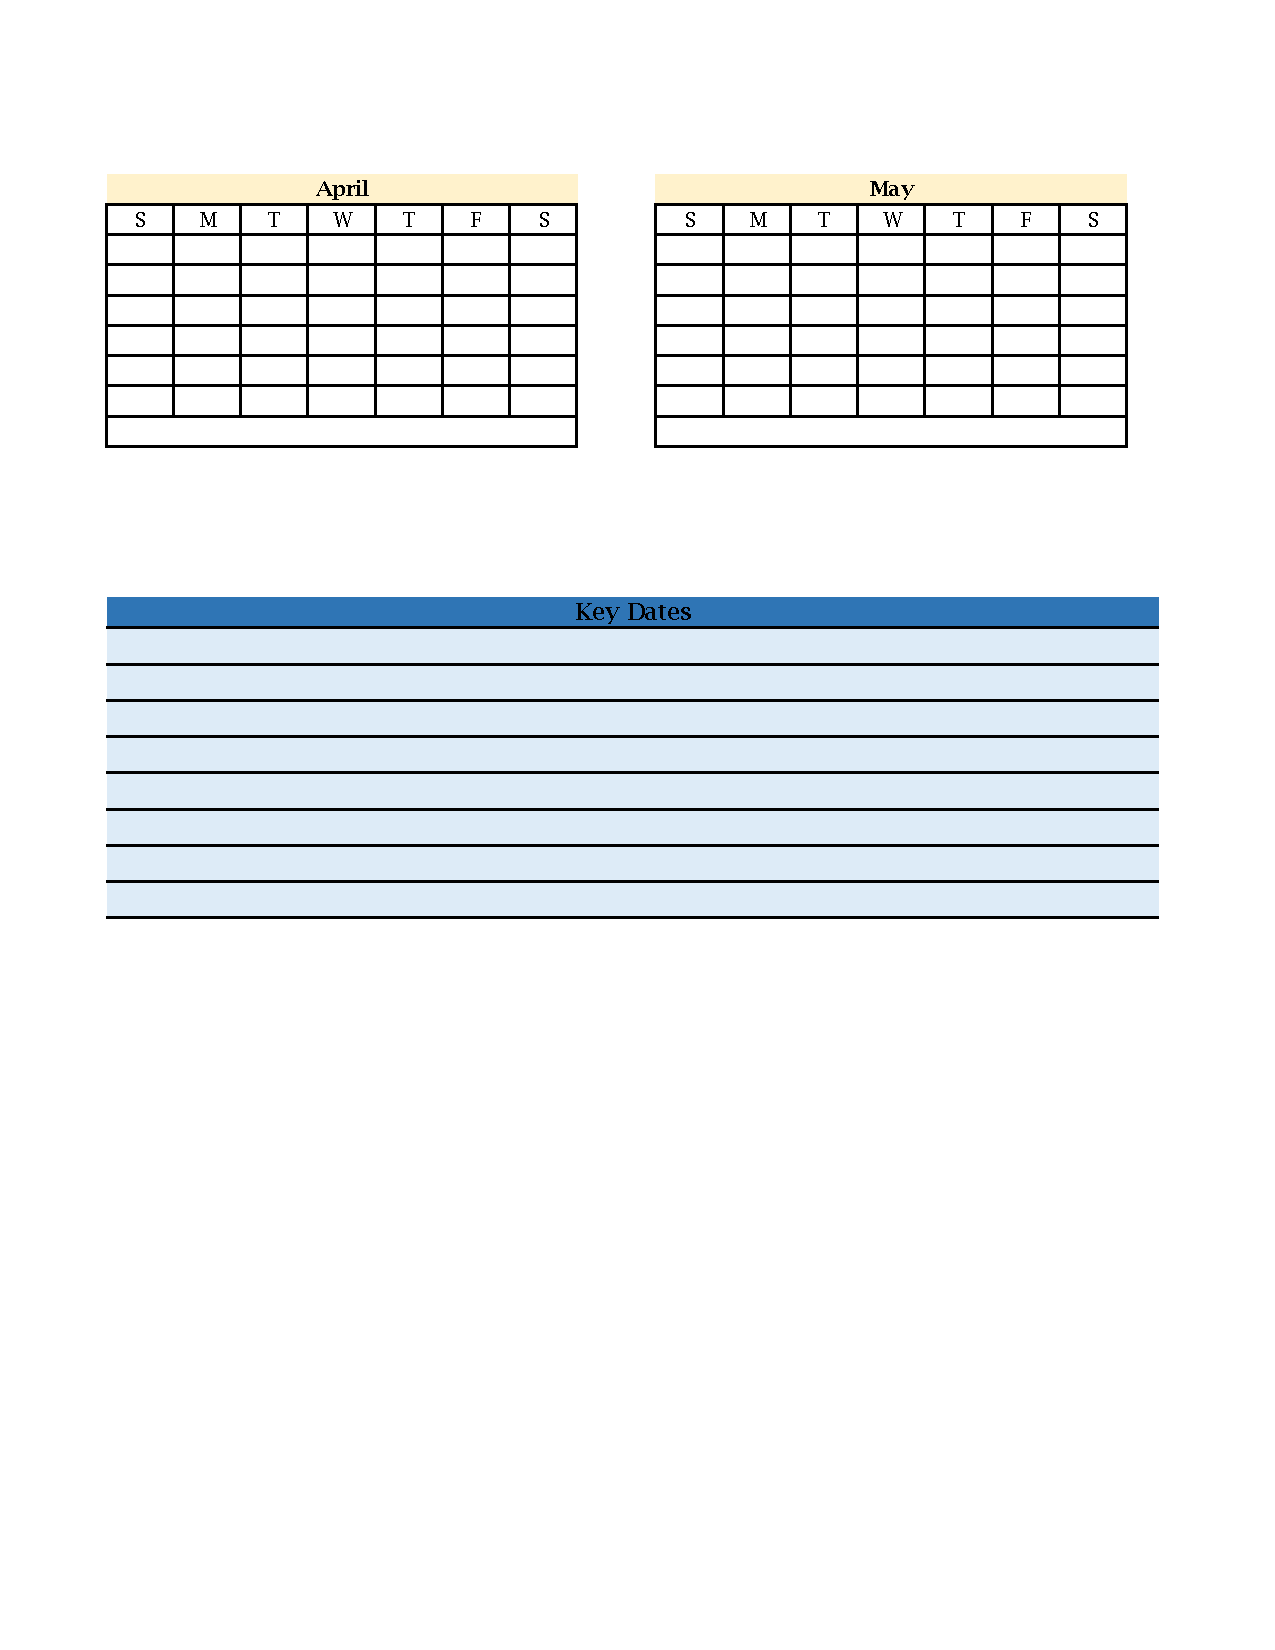
\includegraphics[width=4.5in,height=7in]{Calendar4.pdf}

\end{mybox}
%\input{blank_calendar.tex}
%\input{course_overview.tex} %what days cover what content?
\mypage
\mypage
\addcontentsline{toc}{section}{Lesson Plans}

\vspace{6cm}
\begin{center}
{\Large \textbf{Lesson Plans}}
\end{center} 
\mypage
\Repeat{40}{\addlesson}
\mypage
\mypage
\mypage
\addcontentsline{toc}{section}{Teaching Toolbox}

\vspace{6cm}
\begin{center}
{\Large \textbf{Teaching Toolbox}}
\end{center}
{\setstretch{1}

%% \addtoolboxitem{Title}{What is it?}{Variants}{Uses}

\addtoolboxitem{Timed Think}
{Pose a question, give the students a set time 
to think about the answer silently, then ask the question again and 
call on a student to answer it.}
{Timed group discussion, timed pair
discussion, untimed lecture pause (ie, pause lecture until enough
hands are raised).}
{In the case of a silent class, this will generally
force an answer from the room. In feedback, students often want
more time to think about a problem after it is asked.}

\addtoolboxitem{Think-Pair-Share (TPS)}
{With a question posed, students 
think silently about an answer. Then they pair up, and share their 
response with their neighbour.}
{Explain instead of share, 
Think-Group-Share, Think-Pair-Share 
with a classroom voting system (Think-Vote-Share-Vote), 
repeated Think-Pair-Share-Think-Pair-Share, Think-Pair-Share where during the "Pair" step the student must find a classmate who has a different answer to them.}
{This is the crux of active learning, 
and should be used for simple, conceptual questions, not 
long computational question.}

\addtoolboxitem{Punctuated Lecture}
{A fast-paced lecture, where at the end of 
every slide there is a comprehension-style question, such as 
\enquote{why does this computation work?}, \enquote{explain 
this step}. The question is then worked through using 
\textbf{TPS}.}
{Questions can be posed in an interactive voting system, see also:
\textbf{Going Through the Steps}}
{This is a good technique for getting 
through material that is emphasized in class, as opposed 
to reviewing pre-class material. It combos well with 
timed thinks and TPS.}

\addtoolboxitem{Free-For-All Online Discussion}
{A class-wide open discussion, where 
any student can contribute text or pictures to a forum-style 
tool. This can be done using TopHat, Google Docs, or Quercus.}
{Timed responses, group submission, 
see also: \textbf{Write \& Quiz}, \textbf{Write the Test}, 
and \textbf{1-Minute Essay}.}
{This can be used for getting a lot of ideas 
fast, and to consolidate student solutions for everyone 
to see and use later in studying.}

\addtoolboxitem{1-Minute Essay}
{Students write a 1-minute essay 
linking concepts, explaining a concept, or summarizing 
a concept learned in class. This can be done with 
or without a specific prompt.}
{5-minute essay, 1-minute paragraph, 
writing in groups, 1-minute list, end-of-class summary. See 
also: \textbf{ice cream sandwich}, \textbf{write \& quiz}, 
and \textbf{free-for-all discussion}.}
{This activity is a good conclusion to a 
lecture, module, or other topic. Walking around to pick 
students to read their sentences out loud to their 
neighbours can also be used to build comfort 
within a group.}

\addtoolboxitem{Fill-In Blanks}
{A short, fill-in-the-blanks 
pop-quiz, either on the board, on a slide, or through 
an interactive classroom response system.}
{Giving the word possibilities, see also: \textbf{1-minute essay}}
{This is a good activity to start a 
class or a topic, and to make sure that everyone 
has done the reading, is on the same page, 
and is ready to start learning.}

\addtoolboxitem{Write \& Quiz}
{Students come up with a question, 
then partner up and quiz each other.}
{Larger groups sharing the questions, forcing questions to be
conceptual or computational. See also: \textbf{free-for-all
discussion}, \textbf{write the test}, \textbf{paper passaround}.}
{This is a good activity when there is a lot 
of relatively straightforward material that would take a long 
time to go over, but should be spot-checked. This activity 
also gets students to think about what questions could appear 
on tests.}

\addtoolboxitem{Concept Map}
{A concept map is a directed 
or undirected graph with concepts for nodes and 
edges for connections between them. Edges should be labeled. 
The activity is to make a concept map.}
{Students can get: list of concepts, 
the concept map without edges, or the concept map 
with unlabelled edges.}
{This is an excellent review-session 
tool, as it takes up the entire class, and can cover a 
lot of material. The main goal of the activity is to 
introduce students to the idea, not to finish the map.}

\addtoolboxitem{Critique History \& News}
{A short lesson on the origins 
of the course content, or a news clipping related 
to it. The more primary sources, the better.}
{Having students see the 
primary source and critique it.}
{Some students love this, some hate 
it, but it can be used to show to students that math 
was always difficult, and that other people also 
make mistakes.}

\addtoolboxitem{Going Through the Steps}
{Write a sequence of steps to solve 
a problem, and go through them one by one using other 
teaching-toolbox tools.}
{Handout with steps, allow 
students to find the correct order of the steps. 
See also: \textbf{punctuated lecture}, 
\textbf{think-pair-share}.}
{This is a good activity to use 
to teach students a specific problem-solving strategy.}

\addtoolboxitem{The Tommy Question}
{Tommy writes an incorrect or incomplete solution to a problem, 
and the students need to fix the solution.}
{Use previous exam solutions, have students grade the response, 
let students address their explanation to Tommy}
{This is a good activity to target subtle misconceptions and 
to highlight common pitfalls students may encounter}

\addtoolboxitem{Round Robin}{Students get into groups and take turns highlighting key points from the lecture or course content. Possible variant: \textbf{Playing Darts} - Students shout concepts related to the material, and the 
instructor writes them down on the board. Finish with a follow-up at the end of class outlining what was and wasn't covered in class. 

Pairs well with a \textbf{timed think}}
{This activity can be an opener and a closer, and reminds 
students that they are also responsible for things not covered 
in class.}

\addtoolboxitem{Ice Cream Sandwich}
%(AKA: neapolitan ice-cream)
{Students write three things: something they've 
mastered in the unit, something they're struggling with, and something that was cleared up}{Any triple of questions can work!}{Student reflection, seeing learning as a dynamic process.}

\addtoolboxitem{Draw the Definition/Theorem}{Provide the students with a definition or theorem and have them illustrate this definition or theorem. Their drawing could be of an explicit example which works, or something more general.}{Provide the students with a definition or theorem and a sketch. Have students fill in anything which is missing, and have them colour-code parts of the definition or theorem and colour the corresponding part of the picture that colour as well.}{Allows students to engage with a definition or theorem and build some intuition about the concept.}

\addtoolboxitem{Geogebra Applets}{Geogebra has many free applets available on its platform. It is possible to find many applets which are interactive and allow students to interact with different concepts. Be sure to test out the applet before use to ensure it is what you're looking for!}{There are a variety of different applets available. Some of the applets can be an entire activity on their own, and others can be a supplement to help you illustrate an idea to students.}{Allows students to build intuition behind different concepts in a visual, yet interactive way.}

\addtoolboxitem{Jigsaw}{Break the class into groups and have each group solve a different part of a problem. At the end, every one comes together to synthesize their solutions to solve the main problem.}{This can be used to fill in tables, to see patterns emerging through examples, or to solve a larger problem as a group.}{This can be used to explore theorems or definitions and build intuition.}

\addtoolboxitem{Gameshow}{For review, have large a variety of questions prepared which you will display one at a time. Students will answer questions, and will keep track of their longest streak of correct answers.}{Could have the class break up into teams to play, or change the format to mimic a real game show (for example, Jeopardy).}{A fun way to engage students during a review class before a midterm or final exam.}

\addtoolboxitem{Paper Passaround}{In groups, students write things on papers, and exchange with other groups. The other group reads, and responds on the page.}{Some examples: each group solves one of three problems on the board, and then critiques another group's solution. See also: \textbf{Write \& Quiz}}{This is a good physical writing exercise that 
lets students see and critique how math can be communicated in writing.}

\addtoolboxitem{Run the Test}{Students play the role of the instructor in writing, grading, or helping students during a test-environment. For example, students may be given a solved test to critique, or could be asked to give advice to students before, after, or during the test (see: \textbf{Tommy question})}{An online tool to collect student-made test questions to create a question bank can be useful.}{This exercise can be used to demystify the test, and to highlight common mistakes. See also: \textbf{Write \& Quiz}, \textbf{Free-For-All Online Discussion}}


\mute{
-round robin: four key points from the class [Hannah]
-every group does a different computation/calculation/activity, and then 
it's synthesized together to make a rule/theorem/idea [Yvon]
- Think-Pair-share, then find someone who thinks otherwise, TPS, repeat. [added to think-pair-share]
- Geogebra applet [Yvon - Hannah]
- Gameshow: longest correct answer streak on TopHat. Ask a question, 
somehow track who got a correct answer streak. Students have a goal. [Yvon]
- Split the class into chunks, chunks answer together, and each chunk is 
competing.

\mypage
\subsection*{Ice Cream Sandwich}
(AKA: neapolitan ice-cream)
(students write:
1. Something they've mastered in the unit
2. Something they're struggling with
3. Something that was cleared up)
[Hannah]

\mypage
\subsection*{Paper Passaround}
(I post three questions on the board, 
and groups can choose which to answer. They write answer, and pass 
around to other groups who critique it.) [Hannah]

\mypage
\subsection*{Write the Test}
(this works well with a TopHat discussion or a public document: 
students spend five minutes coming up with possible test questions, 
and then have a resource to study from)

\mypage
\subsection*{Grade A Question}
(give a screenshot of a bad solution, students grade it. 
see: Tommy question)

\mypage
\subsection*{Pre-Class Reflection}

}
}

%% Adds some empty teaching toolbox to fill in your own things

\addblanktoolboxitem
\addblanktoolboxitem
\addblanktoolboxitem
\addblanktoolboxitem
\addblanktoolboxitem

\mypage
\mypage

\vspace{6cm}
\begin{center}
{\Large \textbf{Other Resources}}
\end{center}

\mypage
\addcontentsline{toc}{section}{Targeted Reflection Questions}
\begin{listbox}[width=\textwidth,title={Targeted Reflection Questions}]
  \textbf{
  \begin{enumerate}
    \item What is something that surprised me?
    \item Did any student make the class special?
    \item What teaching strategy went well?
    \item Did something funny happen?
    \item When was the class was engaged/disengaged?
    \item How did the space affect the class?
    \item What did I do that was helpful?
    \item Did something accidental happen?
    \item When did the class feel rushed/slogged?
    \item Expand an activity from the class
    \item How did my body language affect the class?
    \item What mistakes did I make?
    \item What was a good question that was asked?
    \item How did my introduction affect the lesson?
    \item How did my conclusion tie the class together?
    \item A haiku about my class.
    \item What are my students struggling with?
  \end{enumerate}
  }

\end{listbox}

%TODO

\mypage
\addcontentsline{toc}{section}{Critical Incident Questionnaire}
\subsection*{Critical Incident Questionnaire}
\textbf{
One can put this on a google docs survey for the students to complete, TopHat, or paper.  The idea is to give the survey periodically throughout the semester and provide the students feedback on the lecture immediately following the survey.}

\textbf{
A good idea is to use a URL shortener and give the students a short URL.}
\vspace{0.5cm}

\begin{mybox}[width=\textwidth,title=Critical Incident Questionnaire]
\textbf{
\begin{itemize}
    \item At what moment in class this week did you feel most engaged with what was happening?
    \item At what moment in class this week were you most distanced from what was happening?
    \item What action that anyone (teacher or student) took this week did you find most affirming or helpful
    \item What action that anyone took this week did you find most puzzling or confusing?
    \item What about the class this week surprised you the most?
\end{itemize}
}
\end{mybox}

\textbf{
How will you (the instructor) make changes to accommodate the student feedback? The best practice is to provide students with the summary of their responses (i.e. top replies) and indicate what changes you are implementing to address these.
}
\mute{
Critical Incident Questionnaire form:  One can put this on a google docs survey for the students to complete, TopHat, or paper.  The idea is to give the survey periodically throughout the semester and provide the students feedback on the lecture immediately following the survey.
%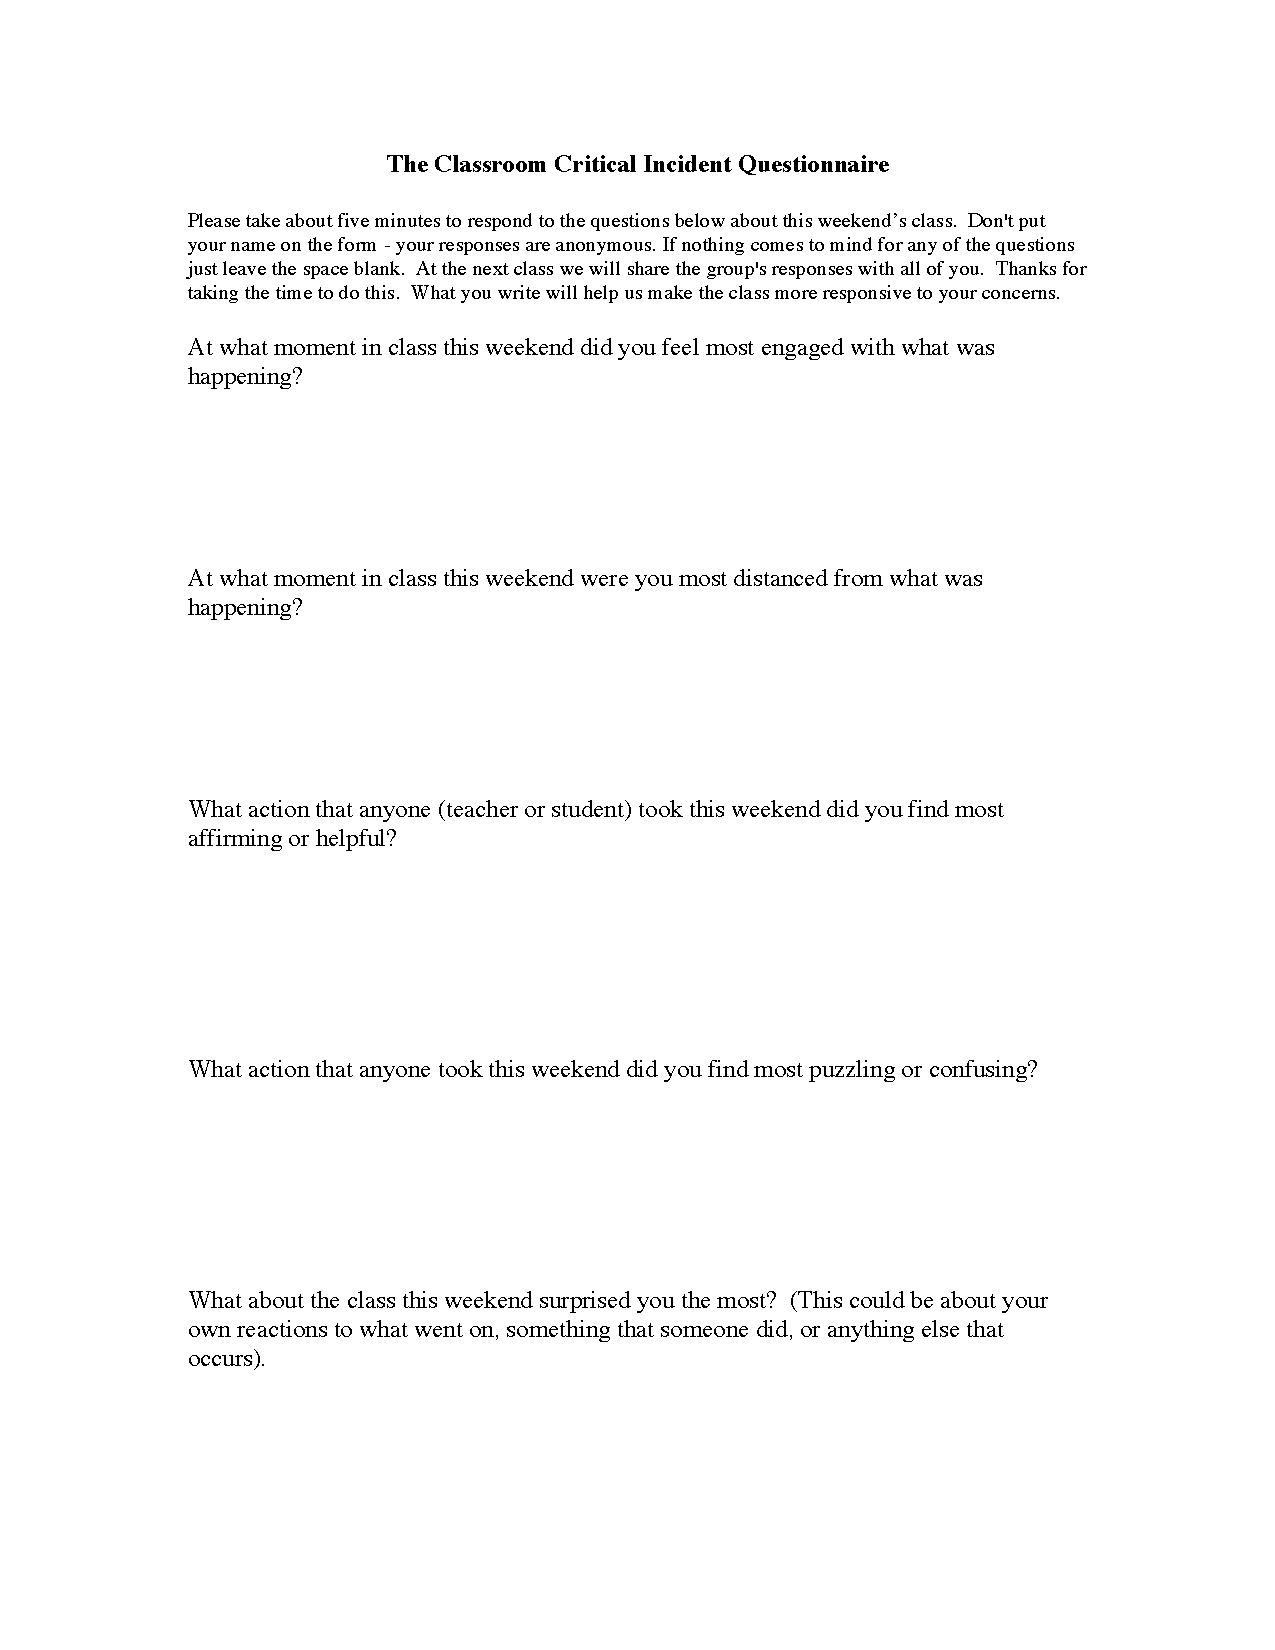
\includepdf[pages=-]{CIQ.pdf}
\subsection*{CIQ Summary of Student Responses}
\begin{center}
  \begin{tabular}{rp{4in}}
    \textbf{Question 1:}& At what moment in class this week did you feel most engaged with what was
happening?\\
        \textbf{Top Response:}& 
    \vspace{1 in}
    \\
    \textbf{Question 2:}& At what moment in class this week were you most distanced from what was
happening? \\
        \textbf{Top Response:}& 
    \vspace{1 in}
    \\
    \textbf{Question 3:}& What action that anyone (teacher or student) took this week did you find most
affirming or helpful \\
        \textbf{Top Response:}& 
    \vspace{1in}
    \\
    \textbf{Question 4:}& What action that anyone took this week did you find most puzzling or confusing?\\
        \textbf{Top Response:}& 
    \vspace{1 in}
    \\
     \textbf{Question 5:}&What about the class this week surprised you the most? (This could be about your own reactions to what went on, something that someone did, or anything else that
occurs).
\\
    \textbf{Top Response:}& 
    \vspace{1 in}
    \\
  \end{tabular}
\end{center}

\subsection*{Changes planned by Instructor}How will you (the instructor) make changes to accommodate the student feedback.  If choosing not to, explain. The best practice is to provide students with the summary of their responses (i.e. top replies) and indicate what changes you are implementing to address these.
\vspace{2.5 inches}

\subsection*{Instructor reflection on any changes made}

\vspace{2.5 inches}
}
\mypage
\addcontentsline{toc}{section}{Resources}
\begin{listbox}[width=\textwidth,title={Phonebook}]
  \textbf{
  \begin{enumerate}
  \item Campus Police: 416-978-2222
  \item Building Related Issues: 416-978-3000
  \item Student Crisis Response: 416-946-7111
  \item Accessibility Services: 416-978-8060
  \item \fillinline{}
  \item \fillinline{}
  \end{enumerate}
  }

\end{listbox}
\begin{listbox}[width=\textwidth,title={Other Resources}]
  \textbf{
  \begin{enumerate}
  \item The Active Calculus Textbook: activecalculus.org
  \item TopHat Field Manual: TODO
  \item \textit{Peer Instruction: A User's Manual}, by Eric Mazur
  \item \textit{Make It Stick: The Science of Successful Learning}, by Peter C. Brown
  \item American Mathematical Society blog on math education: blogs.ams.org/matheducation/
  \item Teaching in higher education podcast:  teachinginhighered.com
  \item Professor Mayes-Tang's Medium page (articles): medium.com/@SMayesTang
  \end{enumerate}
  }
\end{listbox}
\mypage

\begin{listbox}[width=\textwidth,title={Articles, Studies, and Literature}]
\textbf{
\begin{enumerate}
    \item CBMS: Active Learning in Post-Secondary Mathematics Education Statement
    \item \textit{What does active learning mean for mathematicians?}, AMS Notices, B. Braun et al.
    \item \textit{Active learning increases student performance in science, engineering, and mathematics}, by S. Freeman et al.
    \item \textit{Persistent Learning, Critical Teaching: Intelligence beliefs and active learning in mathematics courses}, AMS Notices, B. Braun
    \item \textit{From Lecture to Active Learning: Rewards for all, and is it really so different?}, David Pengally
    \item \textit{What have we learned from calculus reform?  The Road to conceptual understanding}, D. H. Hallett
    \item \textit{Problem Solving: Moving from Routine to Nonroutine and Beyond}, AMS Notices, B. Garelick
    \item \textit{Measuring actual learning versus feeling of learning in response to being actively engaged in the classroom}, L. Deslauriers et al, PNAS, 2019.
\end{enumerate}
}
\end{listbox}
\textbf{Many thanks to Professor Mayes-Tang for her help in compiling this list.}
{\setstretch{1}

\mypage
\subsection*{Teaching Quotes}

%\addcontentsline{toc}{section}{Teaching Quotes}

\myquote{I am not a teacher, but an awakener}{Robert Frost}
\myquote{I never teach my pupils. I only attempt to provide the conditions in which they can learn.}{Albert Einstein}
\myquote{What we learn with pleasure we never forget.}{Alfred Mercier}
\myquote{To teach is to learn twice over.}{Joseph Joubert}
\myquote{I am interested in helping students feel successful; to
attempt to remove the comfort zone of the passive learner and to
empower students to actively engage in their own learning as well as
that of their peers.}{Simon Albon}
\myquote{I believe passionately in David Suzuki's notion of
\enquote{the power of one,} that I can make a difference in my work
with prospective teachers and create a \enquote{ripple effect} in
education. This means I have a responsibility to be a role model as
a scholar, a teacher, and mentor to help my students implement
informed and thoughtful teaching practices, build communities of
inquirers in their classrooms and schools, and become lifetime
learners through ongoing professional development and study.}{Marilyn Chapman}

\mypage
\myquote{You can teach anyone who is interested in teaching to be
a good teacher: to set realistic objectives, to be well organized, to
be clear... What people who become truly exceptional teachers add to
these basic skills is they really truly care that their students
learn.}{Carol-Ann Courneya}
\myquote{An educated person is transformed by what she knows; it
changes her outlook, her horizons, and her habits of mind. To teach
someone is to participate consciously, and carefully, in that
transformation.}{Linda Farr Darling}
\myquote{I let students know that in real life, there's more than one
right answer. My job is to teach them how to approach a problem -- how
to learn, not just what to learn.}{Mary Ensom}
\myquote{I emphasize clarity and planning. Equally important are
a sense of humour and a courteous attitude.}{Keith Farquhar}
\myquote{The thing I enjoy most is teaching first-year courses.
A first-year course is not just an introduction to some subject -- it
is also an opportunity for the instructor to introduce students to his
or her passion for that subject.}{Christopher Friedrichs}

\mypage
\myquote{It is a real privilege to teach students -- an opportunity to
\enquote{turn them on} as opposed to doing the reverse. And the key to
\enquote{turning them on?} I feel it has to do with believing in what you are
selling. For if you don't and would rather be elsewhere, students pick
that up and you impact lessons. So, if there is one quote from me, it
would be: It's not hard to sell something (indeed some\textbf{one}) you believe
in.}{Dan Gardiner}

\myquote{Teaching students less can help them remember more.}{Lee Gass}
\myquote{Students seem to learn best when their curiosity is engaged
and they can feel the link between the material and their own past,
present or future lives. Given this, good teaching is about fostering
curiosity. It is about finding, fueling, and firing up the links and
creating experience within and between learners. Course content exists
to be played with, tossed around until it becomes pertinent.}{Clarissa Green}
\myquote{My basic teaching philosophy is to be enthusiastic about my
subject, honest about potential confusions, and unambiguous in my
explanations}{Chris Orvig}
\myquote{My philosophy of teaching is to provide an atmosphere of
caring and respect for students in order to promote free-thinking and
independent learning.}{Wayne Riggs}

\mypage
\myquote{My philosophy with regard to education is that the teacher
should facilitate the student in their search for knowledge (rather
than deliver the knowledge per se). With this in mind I try to engage
the students in an interactive discussion around the specific subject
matter which they need to know.}{Niamh Kelly}
\myquote{I believe teaching should promote the autonomy of students;
elicit the preoccupations, passions, and lived experience students
bring to the academy; and create a space for articulation and
scholarly inquiry of these elements in their research and in their
writing. My priority is creating a learning environment with
structures that engage student participation and whereby their
participation shapes the learning environment.}{Karen Meyer}
\myquote{I believe that teaching is a creative art in which
evidence-based knowledge is applied toward meeting the learning goals
of learners. I believe that effective teaching is often the spark that
ignites the imagination, possibility, and promise for learners,
including the teacher.}{Barbara Paterson}
\myquote{Listen, respect, and respond to students' points of view; be
excited about mutual engagement in construction of knowledge; love
learning and its complexity. Be curious about and committed to the
possibilities inherent in the intersection of scholarship, mentorship,
and pedagogy.}{Marion Porath}

\mypage
\myquote{If your students are highly intelligent, strongly motivated
and well behaved, it matters little how you teach as they will thrive
anyway. If they aren't, your knowledge, preparation and skill as
a teacher do matter.}{William Webber}
\myquote{UBC is a big place, but it need not be an impersonal one. The
instructor's job is to remember that a big class is not just a sea of
faces, but a group of individuals with different backgrounds,
interests and enthusiasms.}{Christopher Friedrichs}
\myquote{My goal is to present topics with excitement and enthusiasm,
drawing on both work and research experiences to make material
relevant. Once students realize the value of their marketable skills
it increases their desire to master those skills and concepts.}{Wayne Riggs}
\myquote{I teach that a discovery is not simply a eureka moment, but
instead a process where you capture a glimpse of nature exposed,
convince your peers of what you saw and demonstrate utility. Eureka on
its own is merely an observation.}{Stephen W. Scherer}

}

\newpage
\thispagestyle{empty}
\tikz[remember picture,overlay] 
\node[opacity=0.25,inner sep=0pt] at (2.5in,-4.1in)
{
\includegraphics[height=0.9\paperheight]{./Images/Hopf_colour.png}};

\newpage
\thispagestyle{empty}
\tikz[remember picture,overlay] 
\node[opacity=0.25,inner sep=0pt] at (2.5in,-4.1in)
{
\includegraphics[height=0.9\paperheight]{./Images/Hopf_colour.png}};

%\input{references.tex}
\end{document}
